% =====================================================================================
% DA4022 final report -- NeurIPS 2026 template (Overleaf: "Formatting Instructions For
% NeurIPS 2026"). DRAFT: the course requires a human-written report, so the team rewrites
% this text in its own words before submission (see report/README.md).
% Every number is taken from results/ (tables via make_tables.py, figures via make_figures.py).
% =====================================================================================
\documentclass{article}

% [preprint] = non-anonymous version with the author names and the footer
% "Preprint. Work in progress." The default option (main track) is the anonymous
% double-blind submission and would hide the author names; [final] is reserved for
% papers accepted to NeurIPS. Keep the template's neurips_2026.sty unchanged.
\usepackage[preprint]{neurips_2026}

\usepackage[utf8]{inputenc} % allow utf-8 input
\usepackage[T1]{fontenc}    % use 8-bit T1 fonts
\usepackage{amsmath}        % \text, aligned math
\usepackage{graphicx}       % figures
\usepackage{adjustbox}      % tables shrink only if wider than the text
\usepackage{hyperref}       % hyperlinks
\usepackage{url}            % simple URL typesetting
\usepackage{booktabs}       % professional-quality tables
\usepackage{amsfonts}       % blackboard math symbols
\usepackage{nicefrac}       % compact symbols for 1/2, etc.
\usepackage{microtype}      % microtypography
\usepackage{xcolor}         % colors

\title{Quantifying Look-Ahead Bias via Causal, Volatility-Aware Motif Tokenization in Financial Time Series}

% AUTHOR ORDER: change it here only. (The 15 Oct midterm slide listed: Sanidhya Srivastava,
% Arnav Tiku, Devansh Jangid, Karan Malik, Aman Gupta.)
\author{%
  Devansh Jangid \quad Aman Gupta \quad Arnav Tiku \quad Sanidhya Srivastava \quad Karan Malik \\
  DA4022 Course Project \\
  \texttt{github.com/devanshjangid2005/causal-vol-tokenizer}
}

\begin{document}

\maketitle

% ------------------------------------------------------------------ Abstract (~0.25 page)
\begin{abstract}
Byte-pair-encoding (BPE) motif tokenizers for time series are usually validated zero-shot on
held-out datasets. In single-market walk-forward forecasting they can leak post-origin information
in two ways: at fit time, through normalization statistics, merge tables or decoding tables
estimated on test-period data, and at encode time, because rank-ordered BPE is not incremental at
an arbitrary forecast origin. We build a causal reference pipeline for 5-minute BTCUSDT
realized-volatility forecasting (hour-bounded BPE, hourly scale tokens, a causal RoV$\times$SEI gate
and an 855,169-parameter GPT) and switch on one leakage channel at a time against a matched control,
in training and testing alike. Over six walk-forward folds (26,290 hourly test origins, three
seeds), a normalization window that reaches into the forecast horizon lowers QLIKE by 63.39\%
against its matched control (random-effects estimate 62.03\%,
$I^2=0\%$), and it is the only channel that beats the analytic oracle floor of a simulated GARCH
negative control. The merge-table, decoding-table, token-boundary and non-causal-gate channels are
bounded at $+2.84\%$ or less at the one-hour horizon but grow at the one-day horizon, where a
boundary leak can hide partial-token bias. A 2025 holdout, scored once, confirms the normalization
leak ($+73.90\%$).
\end{abstract}

% ------------------------------------------------------------------ 1. Introduction (~0.5 page)
\section{Introduction}

\citet{gotz2026bpe} tokenize time series into motifs: they quantize normalized values into bins,
learn a BPE merge table over the bin sequence and decode generated tokens with conditional tables.
Such tokenizers are usually evaluated zero-shot, on datasets that neither tokenizer nor model has
seen. In walk-forward forecasting on one market, however, every fitted object of the pipeline is
estimated on the series that is later forecast, and each is a possible route for future
information. Leakage has been documented at the level of datasets and correlated series
\citep{meyer2025leakage}, but not channel by channel inside the tokenizer.

Two kinds of leak are possible. Fit-time leaks arise when normalization statistics, the merge table
or the decoding tables are estimated on data that overlap the test period. Encode-time leaks arise
because rank-ordered BPE is not incremental: under the definition of \citet{zhang2026unitok}, which
we apply to BPE, encoding a prefix need not give a prefix of the encoding of the full series.
Tokenizing the context and the horizon once and then cutting at the origin lets the token that
straddles the origin carry future bars, while tokenizing the context alone leaves a possibly partial
final token, which biases next-token prediction \citep{phan2024tokenization}.

We ask which parts of a BPE motif-tokenization pipeline leak post-origin information in walk-forward
volatility forecasting, and by how much each one inflates measured accuracy. Our contributions are:
\begin{itemize}
  \item a per-channel audit of five leakage channels (normalization window, merge table, decoding
        tables, token boundaries, non-causal spectral gate), each switched on alone against a
        matched control in both training and testing;
  \item a measurement of the trade-off between token-boundary leakage and partial-token bias;
  \item a causal tokenizer with hard hour boundaries, hourly scale tokens and a causal
        RoV$\times$SEI gate borrowed from PATK \citep{liao2026patk}, empirically incremental at
        every hour-aligned origin;
  \item a protocol with negative and positive controls, six walk-forward folds, a 2025 holdout
        scored once and seed-averaged robust statistics.
\end{itemize}

% ------------------------------------------------------------------ 2. Method (~0.9 page)
\section{Method}

\begin{figure}[t]
  \centering
  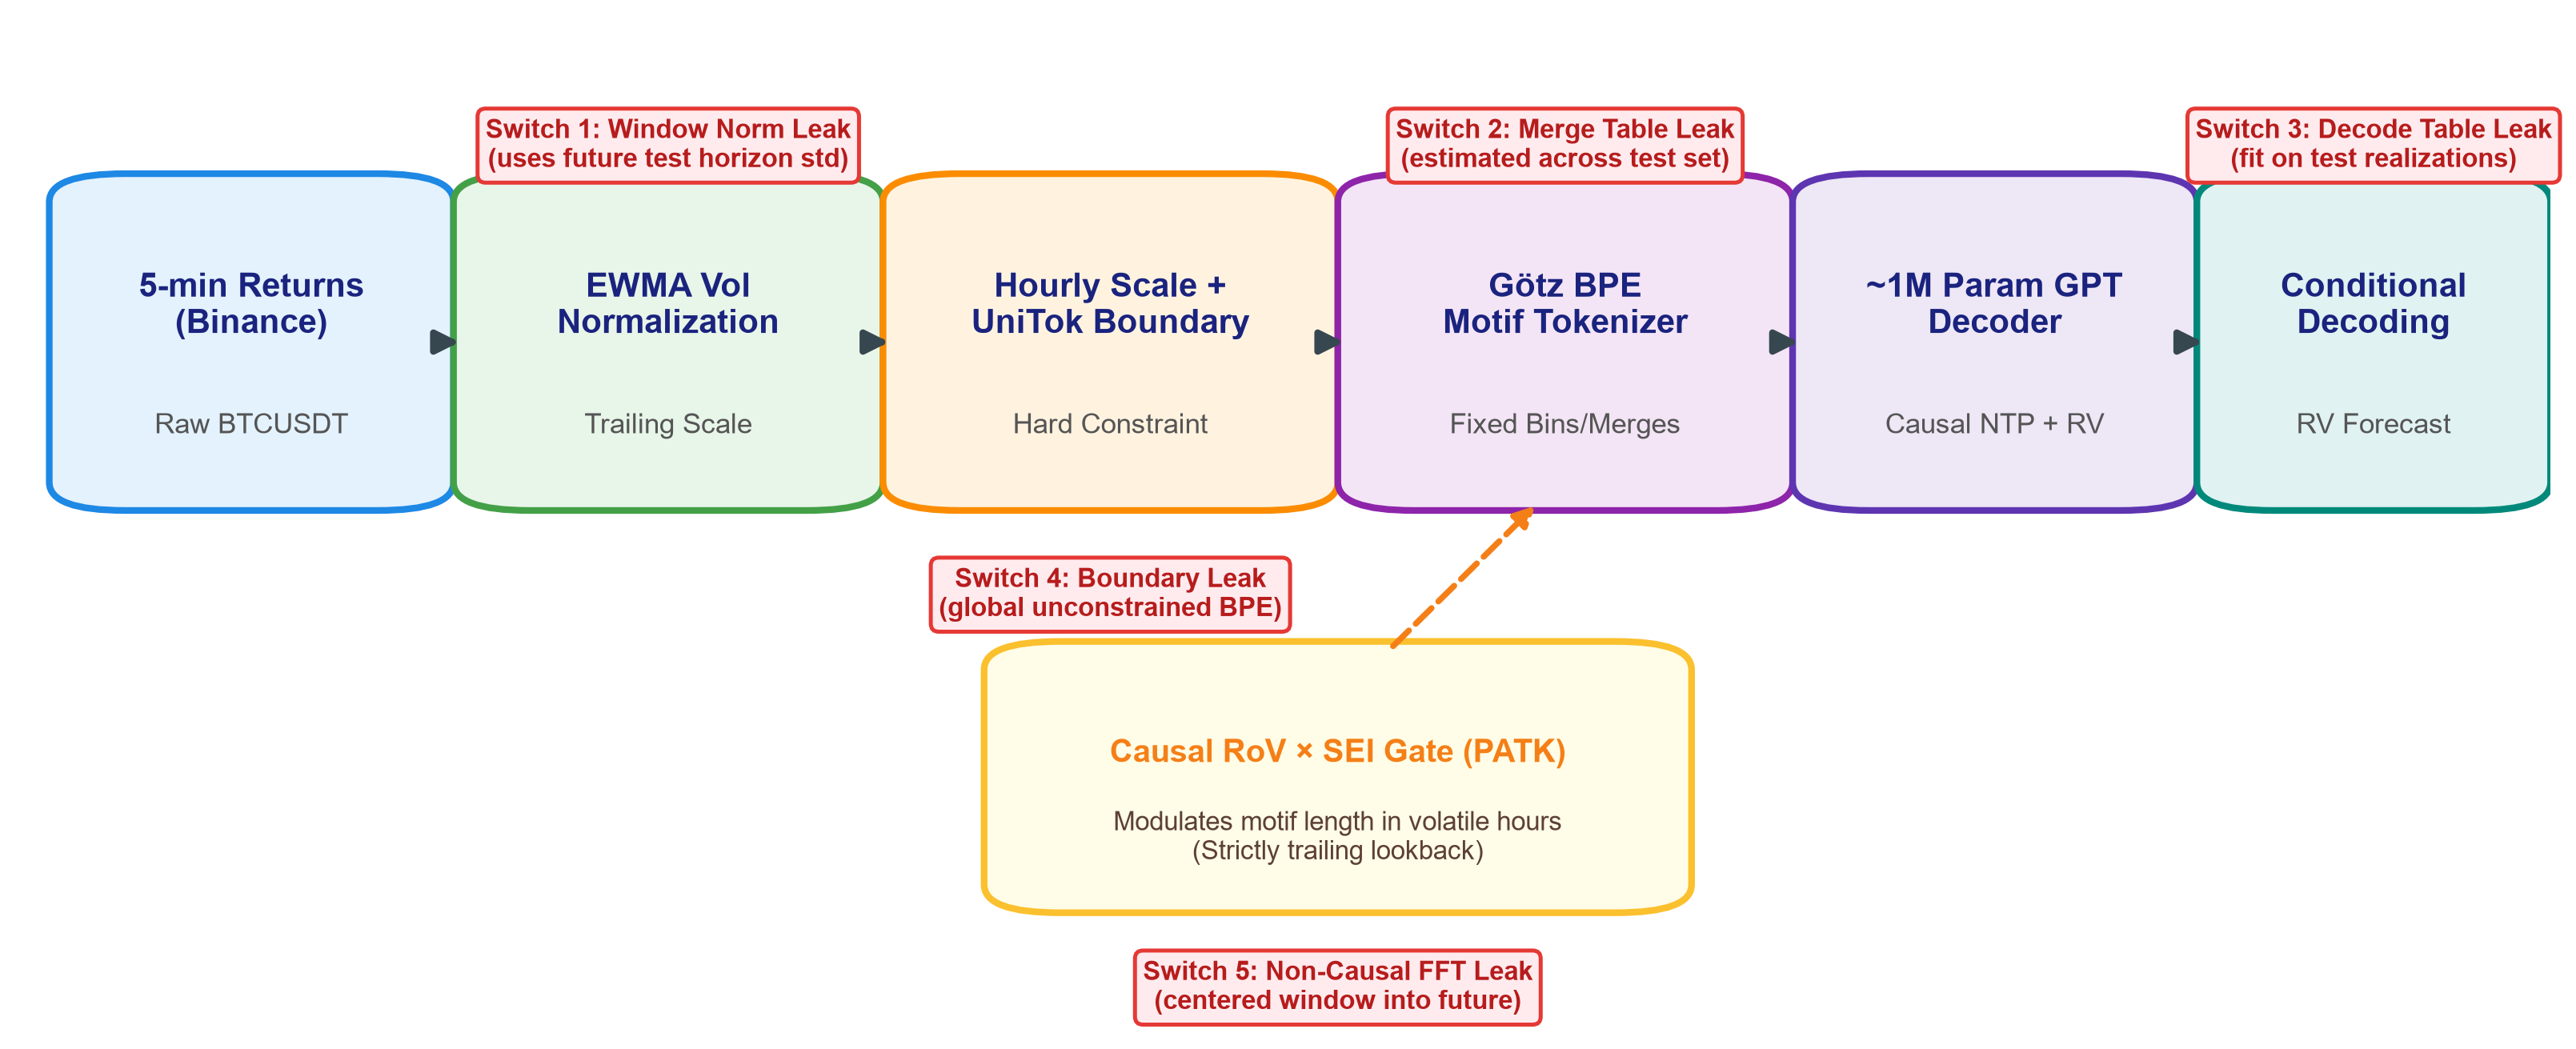
\includegraphics[width=\linewidth]{figures/pipeline_leak_switches.png}
  \caption{Causal reference pipeline and the five leakage switches (red boxes). Each leak arm
  differs from its matched control in one switch, active in both training and testing. The GPT has
  855,169 parameters (the figure rounds this to 1M).}
  \label{fig:pipeline}
\end{figure}

\paragraph{Data and target.}
We use Binance spot 5-minute BTCUSDT bars from January 2021 to December 2025. Log returns $r_t$ are
set to zero across exchange gaps, and each return is normalized by a strictly trailing EWMA
volatility, $\sigma_t^2 = 0.94\,\sigma_{t-1}^2 + 0.06\,r_{t-1}^2$, giving
$x_t = r_t/\max(\sigma_t, 10^{-6})$. A forecast at origin $t$ may use bars up to $t-1$ and targets
the realized variance $\mathrm{RV}_H(t)=\sum_{k=0}^{H-1} r_{t+k}^2$, with $H=12$ (next hour) or
$H=288$ (next day). Origins lie on clock hours with a context of $C=144$ bars (12 hours); an origin
is skipped if any bar in $[t-C, t+H)$ is missing, and training origins are purged so that $t+H$
never reaches the test period.

\paragraph{Causal reference tokenizer.}
Normalized returns fall into 32 uniform bins on $[-4, 4]$. A table of 64 BPE merges is learned on
training data only and applied in rank order \citep{gotz2026bpe}; merges never cross a clock hour,
so encoding is incremental at hour-aligned origins. At each hour start the absolute EWMA volatility
is quantized into one of 16 geometric scale bins on $[10^{-4}, 0.05]$ and emitted as a scale token;
the vocabulary has 112 tokens plus padding. A causal gate scores each hour by RoV$\times$SEI over
the trailing 24 bars (RoV: mean absolute first difference; SEI: share of non-DC spectral energy
within one bin of the dominant frequency; \citealp{liao2026patk}); hours above the 75th percentile
of training-hour scores use only the first 16 merges, giving shorter tokens in volatile periods.
Conditional decoding tables $\mathbb{E}[x_i \mid b_i, b_{i-1}]$ and
$\mathbb{E}[x_i^2 \mid b_i, b_{i-1}]$ are fitted on training data.

\paragraph{Model.}
The forecaster is a decoder-only transformer (4 layers, 4 heads, width 128, feed-forward width 512,
dropout 0.1, 192 positions) with 855,169 parameters. Its direct head regresses $\mathrm{RV}_H/s^2$
for the scale $s$ of the arm's input; its generative head samples 8 continuations at temperature 1
for up to $3H+8$ tokens and sums the decoded conditional second moments over the next $H$ bars.
Training minimizes QLIKE plus $0.5\times$ the next-token cross-entropy with AdamW (learning rate
$10^{-3}$, weight decay $10^{-2}$), batch size 64, gradient clipping at 1 and 5 epochs.

\paragraph{Leakage channels.}
Each leak arm (Figure~\ref{fig:pipeline}) trains its own model with the switch on in training and
testing; only Ch3 reuses the reference model, because decoding tables never enter training.
\begin{itemize}
  \item \textbf{Ch1, normalization window:} the context is scaled by the standard deviation of
        $r_{t-C:t+H}$, which includes the horizon; the control uses $r_{t-C:t}$.
  \item \textbf{Ch2, merge table} and \textbf{Ch3, decoding tables:} fitted on training and test
        data against the train-only reference; Ch3 affects only the generative head.
  \item \textbf{Ch4, token boundaries:} BPE without hour boundaries encodes $[t-C, t+H)$ once and is
        cut when $C$ bars are covered, keeping the token that straddles $t$; the control encodes
        $[t-C, t)$ alone with the same unconstrained tokenizer.
  \item \textbf{Ch5, non-causal gate:} the gate window is centered on each hour, $[s-6, s+18)$, so
        for the last context hour it reaches six bars past the origin.
  \item \textbf{Positive control:} the context is normalized by the true future scale
        $\sqrt{\mathrm{RV}_H(t)/H}$.
\end{itemize}
Partial-token bias is read as the context-only unconstrained arm against the hour-aligned
reference. This comparison changes more than the boundary rule: the unconstrained arm also has no
gate and carries one scale token at the origin instead of twelve hourly ones, so it measures their
joint effect.

% ------------------------------------------------------------------ 3. Setup and statistics (~0.5 page)
\section{Experimental setup and statistics}

\paragraph{Splits.}
Six expanding walk-forward folds all train from January 2021 and test on 2022-Q1, 2022-Q2, 2022-H2,
2023-H1, 2023-H2 and 2024, with 2,160, 2,184, 4,416, 4,330, 4,416 and 8,784 hourly test origins
(26,290 pooled) and 8,657 to 26,163 training origins. The next-day horizon is run on Fold~1 only
(8,496 training and 2,137 test origins, seed 0, direct head). The 2025 holdout trains on 2021--2024
(34,947 origins) and tests on 2025 (8,760 origins) with seed 0; it was scored once, at commit
\texttt{f4ad204}, and a lock file blocks any silent re-scoring. The code was frozen at that commit on
17 November (our midterm plan said 14 November), after fixes for Binance's 2025 timestamps and the
GARCH estimator.

\paragraph{Baselines and tests.}
The baselines are HAR-RV \citep{corsi2009har} with lags of 12, 288 and 2,016 bars, fitted by OLS,
and GARCH(1,1) \citep{bollerslev1986garch} fitted by Gaussian maximum likelihood with
$\alpha+\beta \le 0.9999$; every model is scored on the same origins and target. The loss is QLIKE
\citep{patton2011volatility}, and inflation is
$100 \times (\mathrm{QLIKE}_{\text{control}} - \mathrm{QLIKE}_{\text{arm}})/\mathrm{QLIKE}_{\text{control}}$,
so a positive value means that the leak makes the forecast look better. Moving-block bootstrap
intervals use blocks of 48 origins; the upper end of the 90\% interval is the equivalence bound.
Diebold--Mariano tests \citep{diebold1995comparing} use a Newey--West variance and Holm correction
\citep{holm1979simple} within each family, alongside Giacomini--White \citep{giacomini2006tests} and
TOST tests at $\pm5\%$ of the control's QLIKE. Per-origin losses are averaged over seeds 0--2
before pooling, per-fold estimates are combined by DerSimonian--Laird random effects
\citep{dersimonian1986meta}, and a Model Confidence Set \citep[MCS;][]{hansen2011mcs} with
$\alpha=0.10$ compares the leak-free forecasters. The negative control runs the same pipeline on
simulated GARCH(1,1) data ($\omega=5\times10^{-8}$, $\alpha=0.05$, $\beta=0.93$; 8,748 training and
2,159 test origins), where no causal model can beat the analytic oracle in expectation.

\paragraph{Relation to the midterm.}
A 15 October audit found bugs in our initial prototype. The midterm already withdrew its headline
figures ($+16.6\%$ boundary leak, 84\% boundary mismatch, a GARCH baseline scored on a misaligned
target) and reported post-audit results, which reappear here unchanged. The prototype's Ch1 estimate
($+7.09\%$) is superseded because each arm now trains its own model against a matched control.

% ------------------------------------------------------------------ 4. Results (~2 pages)
\section{Results}

\paragraph{Token-level causality and the negative control.}
On Fold~1 we compare a stream tokenized past the origin and cut at $t$ with the encoding of the
prefix (500 test origins), and replace the bars after $t$ with $5\sigma$ noise (200 origins). The
reference tokenizer matches the prefix at every hour-aligned origin (0\% mismatch, against 31\% at
origins five bars past the hour) and ignores future noise (0\%), so every experiment forecasts from
clock-hour origins. The centered gate of Ch5 changes pre-origin tokens at 57\% of origins, and
unconstrained BPE straddles the origin at 32\% of hour-aligned origins and reacts to future noise at
29.5\%. Compression is modest: 1.40 bars per token at 64 merges. On simulated GARCH data the oracle
floor is 0.1268. Only the Ch1 leak (0.0694 direct, one-sided $p<0.001$; 0.1182 generative,
$p=0.009$) and the positive control fall below it; the reference, the controls and the Ch2--Ch5 arms
all stay above it (Figure~\ref{fig:negctrl}, Appendix~\ref{app:extra}).

\begin{figure}[t]
  \centering
  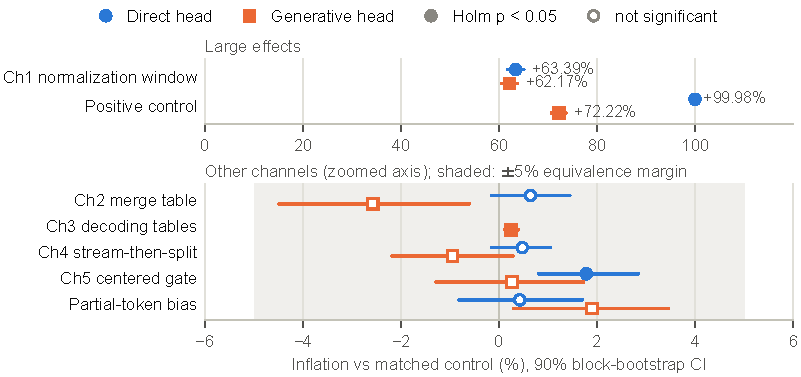
\includegraphics[width=\linewidth]{figures/fig_inflation_folds.pdf}
  \caption{Look-ahead inflation by channel at $H=12$, Folds 1--6 pooled (26,290 hourly origins,
  losses averaged over three training seeds). Markers show inflation against the matched control and
  bars show 90\% moving-block bootstrap intervals, whose upper end is the equivalence bound. Filled
  markers have a Holm-corrected Diebold--Mariano $p<0.05$. The lower panel uses a zoomed axis; the
  shaded band is the $\pm5\%$ TOST margin.}
  \label{fig:folds}
\end{figure}

\paragraph{Inflation per channel at the one-hour horizon.}
Figure~\ref{fig:folds} pools Folds 1--6 (three seeds; full statistics in Table~\ref{tab:robust},
Appendix~\ref{app:extra}). Ch1 dominates: inflation is $+63.39\%$ on
the direct head (90\% CI $+61.77$ to $+65.04\%$) and $+62.17\%$ on the generative head, with a
random-effects estimate of $+62.03\%$ $[58.80, 65.26]$ and no between-fold heterogeneity ($I^2=0\%$;
single folds range from $+54.94$ to $+71.15\%$). The other channels are small. On the direct head,
their 90\% upper bounds limit Ch2 to $+1.44\%$, Ch4 to $+1.05\%$ and Ch5 to $+2.84\%$, and Ch3 is
limited to $+0.39\%$ on the generative head. Ch5 on the direct head ($+1.78\%$, Holm $p=0.034$) and
Ch3 ($+0.24\%$, Holm $p=0.038$) are statistically detectable but tiny, and Ch2 is negative on the
generative head ($-2.58\%$). Partial-token
bias is not significant at this horizon ($+0.42\%$ direct, Holm $p=0.586$; $+1.89\%$ generative,
Holm $p=0.115$). Significance calls for the small channels depend on the seed set (on seed 0 alone,
Ch5 direct is $+3.29\%$ with Holm $p=0.006$), so we report them by their equivalence bounds.

\begin{table}[t]
  \caption{Token-boundary leakage versus partial-token bias (single seed). QLIKE of the hour-aligned
  reference, the unconstrained context-only tokenizer and the stream-then-split tokenizer.
  Partial-token bias compares context-only with the reference (Diebold--Mariano $p$); boundary
  leakage compares stream-then-split with context-only (Holm $p$).}
  \label{tab:tradeoff}
  \centering
  \small
  % Generated by report/make_tables.py from results/ -- do not edit by hand; re-run the script.
\begin{adjustbox}{max width=\linewidth}
\begin{tabular}{lrrrrr}
\toprule
 & \multicolumn{3}{c}{QLIKE (lower is better)} & Partial-token & Boundary \\
\cmidrule(lr){2-4}
Setting & Reference & Context-only & Stream-then-split & bias (\%) & leakage (\%) \\
\midrule
$H{=}288$, Fold 1, seed 0, direct & 0.3128 & 0.3739 & 0.3137 & $-19.53$ ($<$0.001) & $+16.10$ ($<$0.001) \\
2025 holdout, seed 0, direct & 0.4416 & 0.4452 & 0.4494 & $-0.82$ (0.289) & $-0.95$ (0.202) \\
2025 holdout, seed 0, generative & 0.4603 & 0.5538 & 0.4691 & $-20.32$ ($<$0.001) & $+15.30$ ($<$0.001) \\
\bottomrule
\end{tabular}
\end{adjustbox}

\end{table}

\paragraph{Boundary leakage can hide partial-token bias.}
Where partial-token bias is large, the boundary leak recovers almost all of it
(Table~\ref{tab:tradeoff}). At the next-day horizon the context-only tokenizer is 19.53\% worse than
the reference (QLIKE 0.3739 against 0.3128), and tokenizing the stream before splitting brings it
back to 0.3137, a $+16.10\%$ gain over context-only. On the 2025 generative head the pattern
repeats: 0.5538 for context-only and 0.4691 with the boundary leak, against 0.4603 for the
reference; on the 2025 direct head both effects are small. Both large-effect settings use a single
seed, so we report an observed pattern rather than an established effect.

\paragraph{Next-day horizon and the 2025 holdout.}
At $H=288$ (Fold~1, seed 0, direct head) every channel grows: Ch1 reaches $+96.36\%$, Ch4
$+16.10\%$, Ch5 $+7.02\%$ and Ch2 $+5.67\%$, all with Holm $p \le 0.016$. These $p$-values are
probably too small. Hourly origins with 24-hour targets overlap by 23 of 24 hours, while the default
Newey--West bandwidth is about 7 lags, which understates the variance of the loss differential; the
inflation estimates themselves are unaffected. On the 2025 holdout (seed 0;
Figure~\ref{fig:holdout} in the appendix), Ch1 still inflates accuracy by $+73.90\%$ on the direct
head (QLIKE 0.1329 against 0.5093) and by $+68.32\%$ on the generative head. Ch2 changes sign across
heads ($-5.26\%$ direct, $+4.93\%$ generative), consistent with its heterogeneity on the folds, and
Ch5 is not significant on either head.

\paragraph{Leak-free forecasters against the baselines.}
At the one-hour horizon GARCH has a lower loss than HAR-RV in every fold (pooled QLIKE 0.5747
against 0.6811). On the folds, the MCS retains the two leak-free GPT direct forecasters
(context-only 0.5556, reference 0.5580) and excludes GARCH ($p=0.042$). This exclusion depends on
the extra seeds: with seed 0 alone, GARCH stays in the set ($p=0.127$). On 2025 only GARCH remains
(0.4267); the reference GPT direct head (0.4416) beats HAR-RV by 22.08\% but is 3.49\% worse than
GARCH (Diebold--Mariano $p=0.025$). We therefore do not claim that the GPT is the better forecaster;
the study measures inflation, not forecasting skill.

\paragraph{Exploratory extensions.}
On the folds only (Table~\ref{tab:ext}), a window reaching $k$ future bars inflates accuracy
monotonically: $+2.70\%$ for $k=1$ (Holm $p=0.040$), $+6.95\%$ for $k=3$, $+18.38\%$ for $k=6$ (one
seed). ETHUSDT data running through the test period add only $+0.95\%$ (Holm $p=0.188$), whereas
pre-split ETH data add $+3.06\%$ (Holm $p<0.001$), a gain that also reflects twice the optimizer
steps. Token healing improves the same model's generative forecast by $+1.70\%$ (Holm $p=0.295$).

% ------------------------------------------------------------------ 5. Discussion and limitations (~0.6 page)
\section{Discussion and limitations}

\paragraph{Discussion.}
Normalization is the channel to audit first: a window statistic that touches the horizon gives a
large, stable gain at every horizon and on 2025, and it is the only leak that breaks the oracle floor.
The table and encode-time leaks are small at one hour but grow with the horizon. Hour-bounded
tokenization removes the encode-time leak at no measurable cost at $H=12$, whereas a stream-then-split
pipeline can mask a large partial-token cost and look as good as a causal one.

\paragraph{Limitations.}
The study covers one asset at one frequency, with data from 2021 rather than the 2019 start in our
proposal, and a small model trained for five epochs; larger or pretrained models may leak
differently. The next-day results cover one fold, one seed and the direct head (with
anti-conservative $p$-values); the holdout, the dose-response and token healing use one seed, and
the cross-asset arms two. The generative head is noisy ($I^2$ up to 95\% for the small channels).
The partial-token-bias comparison also removes the gate and eleven of the twelve scale tokens, and
token healing uses the standard prefix-compatibility heuristic rather than the exact correction of
\citet{phan2024tokenization}. The gate and scale-token ablations planned at the midterm were not
run, so we cannot separate their contribution to the reference pipeline, and the gate threshold
(the 75th percentile) was not tuned.

% ------------------------------------------------------------------ Acknowledgements (outside the page limit)
\begin{ack}
This report was prepared for the DA4022 course project (instructor: Prof.\ Ayon Borthakur). Code,
results and run logs are available at
\url{https://github.com/devanshjangid2005/causal-vol-tokenizer}.
% Team: add the funding / competing-interest statement here if the instructor requires one.
\end{ack}

% ------------------------------------------------------------------ References (outside the page limit)
{\small
\bibliographystyle{plainnat}
\bibliography{refs}
}

% ------------------------------------------------------------------ Appendix (outside the page limit)
\appendix

\section{Additional results}
\label{app:extra}

All tables and figures in this report are generated from the saved per-origin forecasts in the
repository's \texttt{results/} folder by \texttt{report/make\_tables.py} and
\texttt{report/make\_figures.py}; no experiment was re-run for the report.

\begin{table}[h]
  \caption{Full robust statistics at $H=12$, Folds 1--6 (26,290 origins, losses averaged over seeds
  0--2 per origin). Holm correction is applied within each family (families are separated by the
  rule); RE is the DerSimonian--Laird random-effects estimate across folds with its 95\% interval.}
  \label{tab:robust}
  \centering
  \small
  % Generated by report/make_tables.py from results/ -- do not edit by hand; re-run the script.
\begin{adjustbox}{max width=\linewidth}
\begin{tabular}{llrcrcr}
\toprule
Comparison & Head & Inflation (\%) & 90\% CI (\%) & Holm $p$ & RE across folds [95\% CI] (\%) & $I^2$ (\%) \\
\midrule
Ch1 normalization window & direct & $+63.39$ & [$+61.77$, $+65.04$] & $<$0.001 & $+62.03$ [$+58.80$, $+65.26$] & 0 \\
 & generative & $+62.17$ & [$+60.59$, $+63.71$] & $<$0.001 & $+61.45$ [$+57.38$, $+65.52$] & 0 \\
Ch2 merge table & direct & $+0.64$ & [$-0.14$, $+1.44$] & 0.725 & $+0.39$ [$-0.65$, $+1.43$] & 26 \\
 & generative & $-2.58$ & [$-4.49$, $-0.60$] & 0.134 & $-1.18$ [$-6.63$, $+4.28$] & 91 \\
Ch3 decoding tables & generative & $+0.24$ & [$+0.11$, $+0.39$] & 0.038 & $+0.20$ [$+0.06$, $+0.33$] & 44 \\
Ch4 stream-then-split & direct & $+0.47$ & [$-0.15$, $+1.05$] & 0.725 & $+0.46$ [$-0.16$, $+1.08$] & 0 \\
 & generative & $-0.95$ & [$-2.18$, $+0.29$] & 0.725 & $-0.28$ [$-2.50$, $+1.93$] & 62 \\
Ch5 centered gate & direct & $+1.78$ & [$+0.81$, $+2.84$] & 0.034 & $+1.61$ [$+0.00$, $+3.21$] & 40 \\
 & generative & $+0.26$ & [$-1.28$, $+1.73$] & 0.758 & $+0.32$ [$-5.53$, $+6.18$] & 95 \\
Positive control & direct & $+99.98$ & [$+99.96$, $+99.98$] & $<$0.001 & $+99.98$ [$+95.79$, $+104.16$] & 0 \\
 & generative & $+72.22$ & [$+70.68$, $+73.64$] & $<$0.001 & $+71.60$ [$+64.09$, $+79.11$] & 44 \\
\midrule
Partial-token bias & direct & $+0.42$ & [$-0.82$, $+1.70$] & 0.586 & $+0.02$ [$-1.59$, $+1.63$] & 24 \\
 & generative & $+1.89$ & [$+0.29$, $+3.45$] & 0.115 & $+2.65$ [$-3.13$, $+8.42$] & 90 \\
\bottomrule
\end{tabular}
\end{adjustbox}

\end{table}

\begin{figure}[h]
  \centering
  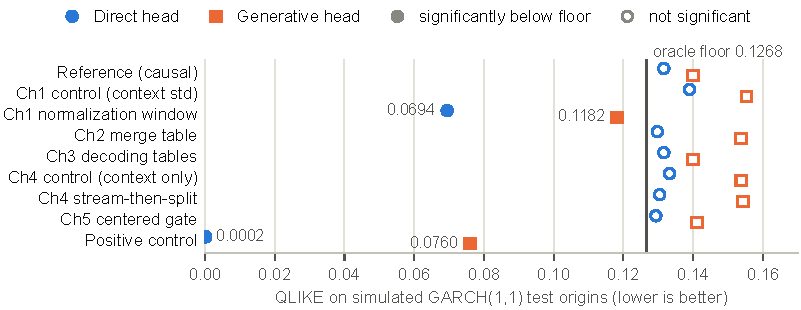
\includegraphics[width=\linewidth]{figures/fig_negative_control.pdf}
  \caption{Negative control on simulated GARCH(1,1) data (seed 0): QLIKE of every arm on the test
  origins against the analytic oracle floor (vertical line, 0.1268). Filled markers lie
  significantly below the floor (one-sided Diebold--Mariano $p<0.05$); only the Ch1 normalization
  leak and the positive control do. The other arms score 0.1293--0.1389 (direct) and
  0.1400--0.1553 (generative); fitted GARCH scores 0.1268 and HAR-RV 0.1322.}
  \label{fig:negctrl}
\end{figure}

\begin{figure}[h]
  \centering
  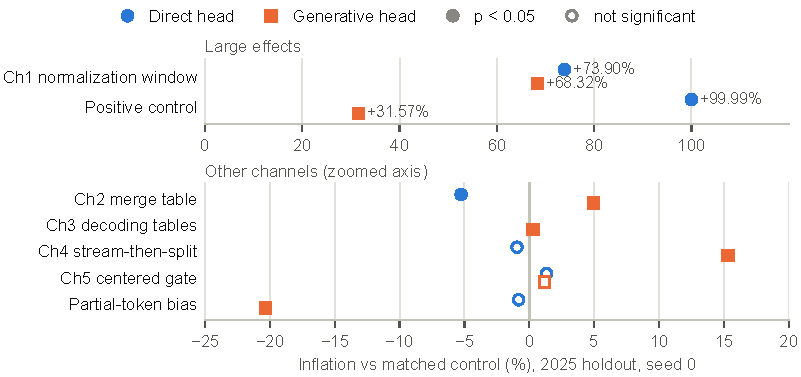
\includegraphics[width=\linewidth]{figures/fig_inflation_holdout.pdf}
  \caption{2025 holdout, scored once (seed 0, 8,760 origins): inflation by channel against the
  matched control. Filled markers have $p<0.05$ (Holm-corrected for the leak channels,
  Diebold--Mariano for partial-token bias).}
  \label{fig:holdout}
\end{figure}

\begin{table}[h]
  \caption{Exploratory extensions (Folds 1--6 only; the 2025 holdout is not used). Seeds give the
  number of training seeds for the arm and its control; Holm correction is applied within each
  block.}
  \label{tab:ext}
  \centering
  \small
  % Generated by report/make_tables.py from results/ -- do not edit by hand; re-run the script.
\begin{adjustbox}{max width=\linewidth}
\begin{tabular}{llcrcr}
\toprule
Comparison & Head & Seeds & Inflation (\%) & 90\% CI (\%) & Holm $p$ \\
\midrule
Ch1 dose: $k{=}1$ future bar & direct & 1/3 & $+2.70$ & [$+0.76$, $+4.92$] & 0.040 \\
Ch1 dose: $k{=}3$ future bars & direct & 1/3 & $+6.95$ & [$+5.31$, $+8.58$] & $<$0.001 \\
Ch1 dose: $k{=}6$ future bars & direct & 1/3 & $+18.38$ & [$+13.92$, $+22.60$] & $<$0.001 \\
Ch1 dose: $k{=}12$ (= Ch1) & direct & 3/3 & $+63.39$ & [$+61.77$, $+65.04$] & $<$0.001 \\
\midrule
ETH through test vs ETH to split (leak) & direct & 2/2 & $+0.95$ & [$+0.16$, $+1.78$] & 0.188 \\
ETH through test vs ETH to split (leak) & generative & 2/2 & $+1.02$ & [$-0.53$, $+2.50$] & 0.287 \\
ETH to split vs BTC only (more data) & direct & 2/3 & $+3.06$ & [$+2.21$, $+3.91$] & $<$0.001 \\
ETH to split vs BTC only (more data) & generative & 2/3 & $+1.89$ & [$+0.02$, $+3.65$] & 0.188 \\
\midrule
Plain unconstrained vs reference & generative & 1/3 & $+0.12$ & [$-2.04$, $+2.17$] & 0.926 \\
Healed vs plain (same model) & generative & 1/1 & $+1.70$ & [$+0.07$, $+3.38$] & 0.295 \\
Healed unconstrained vs reference & generative & 1/3 & $+1.82$ & [$-0.39$, $+4.05$] & 0.367 \\
\bottomrule
\end{tabular}
\end{adjustbox}

\end{table}

% The NeurIPS paper checklist (\input{checklist.tex} in the template) is not included: ask the
% instructor whether the course report needs it. If it does, add it here after a \newpage.
% \newpage
% \input{checklist.tex}

\end{document}
